Tässä luvussa esitetään perusteet ja tarvittavat tiedot hyväksymistestauksesta, johon testauksen tasoista tässä diplomityössä keskitytään.
Ensin esitetään hyväksymistestauksen tarkoitus, jonka jälkeen keskitytään hyväksymistestausvetoiseen kehitykseen ja sen esittelemiseen ohjelmistotuotannollisena menetelmänä.
Hyväksymistestausvetoisen kehityksen jälkeen käydään läpi tässä diplomityössä käytettyä ja lähes de facto testialustaa, Robot frameworkia, hyväksymistestauksen testitapauksien rakentamiseen.
Robot frameworkin perusteiden jälkeen esitetään hyväksymistestauksen testitapauksien laatiminen käyttäen Robot frameworkia sekä esitetään web-sovelluksien erityispiirteitä jotka on huomioitava hyväksymistestauksessa.
Hyväksymistestaksen perusteiden ymmärtämistä tarvitaan työn toteutusvaiheessa, jossa esitetään korkealla tasolla asiakasyritykselle toteutettua hyväksymistestausta ja sen automaatiota.
Lopuksi esitetään yleisestikin ottaen testitapauksiin tärkeästi liittyvä priorisointiongelma ja käydään läpi sen eri ratkaisumalleja, keskittyen erityisesti tässä diplomityössä myöhemmin esitettävään priorisointiin painotetun verkon avulla.

\section{Hyväksymistestauksen tarkoitus} \label{ch:08_hyvaksymistestauksen_tarkoitus}

  Hyväksymistestauksen tarkoituksena on varmistaa toteutettavan ohjelmiston vaatimusten toimivuus erityisesti käytännön tilanteissa siten, että voidaan varmistaa vastaako ohjelmisto loppukäyttäjän tarpeita.
  Hyväksymistestaus antaa vastauksen siihen, toimiiko toteutettu järjestelmä loppukäyttäjän tarpeiden mukaisesti ja loppukäyttäjän näkökulmasta oikein.
  Hyväksymistestauksen sanotaan olevan muodollista testaamista, jossa käyttäjän tarpeet, vaatimukset ja liiketoimintaprosessit otetaan huomioon selvittäessä täyttääkö järjestelmä hyväksymisen kriteerit ja sallii käyttäjän, asikkaiden tai muun autorisoidun tahon päättää hyväksytäänkö järjestelmä \parencite{istqb_glossary_nodate}.
  Ohjelmistotestauksen tekniikoiden näkökulmasta hyväksymistestaus on mustalaatikkotestausta, eli sitä testataan tietämättä sen teknisestä toteutuksesta.
  Hyväksymistestauksen painoarvo on asiakaperusteisessa vaatimusmäärittelyssä ja loppukäyttäjän tarpeiden kartoittamisessa.
  Testiautomaation osalta hyväksymistestausta varten voidaan rakentaa testitapaukset, joiden avulla voidaan keskittyä varmistamaan loppukäyttäjille tarpeellisten toimintojen toteutuminen testitapauksien suorittamisen jälkeen.
  Hyväksymistestauksen osalta testitapauksia voidaan toteuttaa niin sanotulla päästä päähän -periaatteella, jossa testattavaa järjestlemää testataan siten kuin loppukäyttäjä sitä käyttää.
  Hyväksymistestauksessa ei anneta suurta painoarvoa kosmeettisille tai kirjoitusvirheille, vaan pyritään selvittämään loppukäyttäjille oleellisten ja tarpeellisten toimintojen toteutuminen.

  Hyväksymistestaus on aiemmin esitetyistä testauksen tasoista \ref{ch:07_testauksen_tasot} viimeinen ja sen suorittamisen jälkeen saadaan tieto siitä onko järjestlemä toteutuksen osalta sellaisenaan valmis julkaistavaksi.
  Perinteisesti hyväksymistestauksen lähtökohtia ovat selvät hyväksymisvaatimukset sekä julkaisukelpoinen toteutus joka voi sisältää vain kosmeettisia virheitä.
  Hyväksymisvaatimukset voivat olla esimerkiksi liiketoiminnallisia käyttötapauksia, prosessivirtauskaavioita sekä ohjelmiston vaatimusmäärittely.
  Testiautomaatiota varten käytettävästä testialustasta riippuen hyväksymistestauksen käyttötapaukset voidaan muodostaa joko osittain tai suoraan testitapauksiksi.
  Hyväksymistestaukseen usein osallistuu ohjelmistokehittäjien lisäksi myös muut sidosryhmät ja loppukäyttäjät.
  Keskeistä on, että loppukäyttäjiltä hankitaan tieto tarvittavista ja toteutettavista ominaisuuksista, kun taas muut sidosryhmät kuten esimerkiksi johtoryhmä voivat tehdä liiketoiminnallisia päätöksiä hyväksymistestauksen onnistumisen osalta ja esimerkiksi peruuttaa julkaisun.
  Hyväksymistestaus antaa mahdollisuuden korjata usein liiketoiminnalisestakin näkökulmasta merkittävät toiminalliset virheet ennen järjestelmän julkaisua loppukäyttäjille.

  Kehittäjien käsitys järjestelmän toiminnallisuudesta ja sen vaatimuksista voi olla usein hyvinkin erilainen kuin loppukäyttäjien.
  Hyväksymistestauksen avulla voidaan tätä lievittää tätä ongelmaa, ja saattaa ohjelmistokehittäjät loppukäyttäjien kanssa vaatimusmäärittelyn suhteen samalle sivulle.
  Testiautomaation avulla toteutettavalla toistuvalla hyväksymistestauksella varmistetaan, että järjestelmä toteuttaa loppukäyttäjän tarpeet vielä järjestlemään tehtyjen muutoksien jälkeenkin.
  Hyväksysmistestauksen testitapaukset tarkoituksenmukaisesti heijastavat suoraan loppykäyttäjien tarpeita, joka on iso etu sillä sen avulla ohjelmistokehittäjät ja muut sidosryhmät voivat tehokkaasti varmistaa järjestlemän valmiuden ja tilan.
  Hyväksymistestauksella siis saadaan katsaus ohjelmiston valmiudesta sen vaatimuksiin ja loppukäyttäjien toiminnallisiin tarpeisiin nähden.

\section{Hyväksymistestausvetoinen kehitys} \label{ch:08_hyvaksymistestausvetoinen_kehitys}

  Hyväksymistestausvetoisen kehityksen (englanniksi: ATDD, acceptance test driven development) tarkoituksena, kuten testausvetoisessakin kehityksessä \ref{ch:07_testausvetoinen_kehitys} on toteuttaa ohjelmistotuotannollinen prosessi laatien toistettavasti suoritettavat testitapaukset ennen ohjelmiston varsinaista toteutusta.
  Hyväksymistestausvetoisessa kehityksessä tämä tarkoittaa käytännössä sitä, että ennen toteutusta luodaan tarvittavat ohjelmiston asiakasvaatimuksia palvelevat hyväksymistestit, jotka ohjelmiston on tarkoitus läpäistä sen julkaisemisen hyväksymiseksi.
  Hyväksymistestausvetoisen kehityksen sanotaan olevan yhteistyöhön perustuva lähestymistapa kehitykseen, jossa tiimi ja asiakkaat käyttävät asiakkaiden oman ympäristön kieltä ymmärtääkseen heidän vaatimukset, jotka muodostavat pohjan komponentin tai järjestelmän testaamiseen \parencite{istqb_glossary_nodate}.
  Tarvittavat ohjelmiston hyväksymistestit suoritetaan iteratiivisesti ohjelmistokehitysprosessin aikana ja se tarkoittaa käytännössä jatkuvan integraation \ref{ch:07_jatkuva_integrointi} ottamista käyttöön ohjelmistokehityksessä.
  Hyväksysmistestausvetoinen kehitys on erittäin hyödyllinen ohjelmistokehityksessä käytetty menetelmä, sillä kehitysvaiheessa on aina tarkasti tiedossa vastaako ohjelmiston tila asiakasvaatimuksia ja kuinka hyvin se niiden täyttämisessä onnistuu.

  \begin{figure}[H]
    \centering
    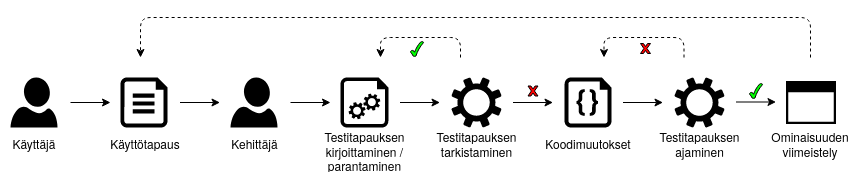
\includegraphics[width=0.8\textwidth]{assets/hyvaksymistestausvetoinen-kehitys.png}
    \caption{Hyväksymistestausvetoisen kehityksen vaiheet}
    \label{fig:hyvaksymistestausvetoinen-kehitys}
  \end{figure}

  Hyväksymistestausvetoinen kehitys voidaan luokitella ketteräksi ohjelmistokehitysmenetelmäksi, kuten sen yläkäsitteenä oleva testausvetoinen kehityskin \ref{ch:07_testausvetoinen_kehitys}.
  Hyväksymistestausvetoinen kehitys on testausvetoisen kehityksen kanssa perusperiaatteeltaan samanlainen, mutta ennen ohjelmistokehityksen aloitusta asiakasvaatimukset kartoitetaan ja ohjelmiston hyväksyttävyys määritetään.
  Hyväksymistestitapaukset kirjoitetaan testausvetoisen kehityksen mukaisesti ensin ja ohjelmistokehitys itsessään noudattaa iteratiivisesti testausvetoista kehitystä, vaikkakin hyväksymistestaus itsessään on perinteisesti vaatinut lähes valmista järjestlemää.
  Asiakasvaatimukset määritetään usein käyttötapauksien muotoon, ja riippuen testialustasta ne voidaan kirjottaa testitapauksien muotoon niitä vahvasti hyödyntäen.
  Hyväksymistestausvetoisessa kehityksessä ohjelmistokehitystä siis ohjaavat asiakasvaatimukset ja loppukäyttäjien tarpeiden toteutuminen, jotka ovat hyvin usein toiminallisia vaatimuksia.
  Hyväksymistestausvetoisessa kehityksessä mitataan jatkuvasti iteroiden käyttötapauksien muodossa validoitavien haluttujen ominaisuuksien toteutumista.
  Perusperiaate on kirjoittaa asiakasvaatimus tai käyttötapaus testitapauksen muotoon, toteuttaa testitapaus, ajaa testitapaus läpäisemättömänä, toteuttaa ominaisuus, ajaa testitapaus läpäisevänä, refaktoroida toteutus ja siirtyä takaisin seuraavaan käyttötapaukseen.
  Käyttötapaus koostuu rakenteellisesti usein tilanteesta, motivaatiosta ja halutusta lopputuloksesta.
  Esimerkki käyttötapauksesta voi olla: \emph{käyttäjänä, haluan sisäänkirjautumisen jälkeen voida avata premium ominaisuudet tekemällä sovelluksensisäisen oston}.

  Hyväksymistestausvetoisessa kehityksessä hyväksymistestit on hyödyllistä pilkkoa pieniin hallittaviin kokonaisuuksiin, jolloin voidaan iteratiivisesti toteuttaa valmiiksi tietyn testitapauksen mukainen ominaisuus, joka vastaa jotakin käyttötapausta tai loppukäyttäjän tarvetta.
  Hyväksymistestauksessa testitapaus voi olla esimerkiksi käyttäjän tietojen muuttuminen varmistaminen, kuten tason läpäiseminen pelisovelluksessa, joka muuttaa käyttäjän edistystä.
  Hyväksymistestausvetoisen kehityksen tarkoituksena menetelmänä on onnistua vastaamaan loppykäyttäjän tarpeisiin tehokkaasti ja hyvin ottamalla tarpeet huomioon jo ennen toteutuksen aloittamista.
  Menetelmän avulla myös luodaan ymmärrystä ohjelmistotuotteen valmiuden määritelmästä kun eri sidosryhmän voidaan saada sen suhteen samalle aaltopituudelle.
  Hyväksymistestausvetoinen kehitys on lisäksi erittäin hyödyllistä, sillä jatkuva testaaminen antaa mahdollisuuden haluttujen ominaisuuksien toteutumisen validoimiselle menetelmän jokaisen iteraation koontiversiossa.

\section{Web-sovelluksien erityispiirteet} \label{ch:08_websovelluksien_erityispiirteet}

  Web-sovelluksilla on omia erityispiirteitä, jotka vaikuttavat testitapauksien laatimiseen.
  Nykypäivänä web-sovellukset ovat kasvaneet kompleksisuudessa ja front-end puolen toteutuksesta tarkasteltuna web-sovellukset usein muistuttavat jo perinteisiä työpöytäsovelluksia.
  Web-sovelluksia päivitetään nykyään tiheään tahtiin ja niille on suuri tarve luoda testiautomaatiota, jota hyödyntäen voidaan varmistaa että ne toimivat oikein muutoksien jälkeenkin.

  Hyväksymistestauksen priorisoimisen osalta tärkeä web-sovelluksien erityispiirre liittyy käyttöliittymiin ja dokumenttiobjektimalliin, DOM.
  Dokumenttiobjektimallin avulla verkkoselaimet renderöivät käyttöliittymän ja siinä näkyvän sisällön.
  Tämän lisäksi dokumenttiobjektimalli mahdollistaa käyttöliittymässä olevien elementtien valitsemisen, jota hyödynnetään myös testitapauksien kirjoittamisessa.

  Navigointi ja navigointiketjut ovat myös yksi web-sovelluksien erityispiirre.
  Historiallisesti verkkosivuilla navigointi tapahtui niin kutsuttujen hyperlinkkien avulla, verkkosivujen itse ollessa hypertekstiä.
  Tämä historiallinen lähestymistapa on edelleen käytössä ja web-sovelluksissa on lähes poikkeuksetta useita hyperlinkkejä joiden avulla navigoiminen luo erityisiä navigointiketjuja, joissa edelliseen sivuun tiedetään palata.
  Hyperlinkkien avulla tapahtuva navigointi ja navigointiketjut on erityispiirre, joka on hyvä tiedostaa myös hyväksymistestauksen testitapauksia rakentaessa.

  Web-sovelluksien syötteet ja niiden yhteyteen liittyvä tietoturva ovat myös yksi niiden erityispiirre joka vaatii suurta huomiota.
  Web-sovelluksien syötteisiin on perinteisesti liittynyt paljon haavoittuvuuksia, kuten esimerkiksi XSS-hyökkäykset ja SQL-injektiot.
  Web-sovelluksien hyväksymistestauksen testitapauksiin on hyvä sisällyttää syötteisiin liittyvää testaamista, joissa tietoturva pidetään mielessä.

  Erilaisia web-sovelluksen loppukäyttäjien asiakasympäristöjä on huikean paljon, joka kannustaa moniselaimellisen testauksen rakentamiseen.
  Näissä ympäristöissä on omat verkkoselaimensa, näyttöresoluutio ja selainasetukset, jotka saavat saman sovelluksen toimimaan eri tavoilla eri ympäristöissä ja luovat siten usein jopa päänvaivaa ohjelmistokehittäjille.
  Etenkin web-käyttöliittymiin keskittyessä testitapauksiin on hyvä sisällyttää erilaisia näyttöresoluutioita, kuvankaappauksien ottamista ja selainasetuksista esimerkiksi Javascript-ominaisuuksien estäminen.

  Web-sovelluksien käyttöliittymien testaaminen ja yleisestikkin ottaen käyttöliittymien testaaminen on perinteisesti tapahtunut manuaalisesti.
  Nykyään web-sovelluksia voidaan testata niin sanotun päätteettömän testauksen keinoin.
  Web-sovelluksien päätteettömässä testauksessa verkkoselaimen, näyttöresoluution ja selainasetuksien muodostamaa asiakasympäristö rakennetaan virtualisoinnin avulla.
  Virtualisoinnista vastaa joko verkkoselain itse tai voidaan käyttää UNIX järjestelmissä x-näyttöpalvelimen protokollan toteuttavaa virtualisointiratkaisua, esimerkiksi Xvfb.
  Virtualisoitu asiakasympäristö rakennetaan siten, että se päätteettömänä vastaa täysin päätteellistä vaihtoehtoa, ja siitä voidaan ottaa esimerkiksi kuvankaappaus vaikka mitään ihmisen astittavaa ei ole näkyvillä.

\section{Hyväksymistestauksen työkaluja} \label{ch:08_hyvaksymistestauksen_tyokaluja}

  Tässä kappaleessa esitetään diplomityötä tehdessä käytettyjä ja osin myös varsin yleisiä testiautomaation mahdollistavia työkaluja, kukin omassa alikappaleessaan.
  Ensin esitetään hyväksymistestauksen automatisoimisen kannalta kaikista tärkeimmät työkalut, eli testikehyksenä käytettävä Robot framework ja web-sovelluksien interaktioiden automatisoimisen mahdollistava Selenium kirjasto.
  Lisäksi esitetään kolme muuta tärkeää työkalua joiden avulla voidaan rakentaa kokonainen ohjelmistotuotannon prosessiin intergroitavissa oleva hyväksymistestausjärjestelmä.
  Toteutuksessa GoCD vastaa jatkuvan integroinnin tarjoamisesta, Xvfb vastaa päätteettömän testauksen tarjoamisesta ja Docker vastaa työkalujen virtualisoimisesta ja säiliöinnistä, jolloin työkaluista saadaan luotua yhtenäinen kokonaisuus.

  \subsection{Robot Framework} \label{ch:08_robot_framework}

    Robot framework on geneerinen avoimen lähdekoodin testausalusta hyväksymistestaukseen, hyväksymistestausvetoiseen kehitykseen ja robotisten prosessien automaatioon \parencite{noauthor_robot_nodate}.
    Testialustana Robot frameworkilla on helposti ymmärrettävä, luettava ja selkeä avainsanaperustainen syntaksi.
    Testialustan etuna on helppo lähestyttävyys ja sen pohjalle rakennettujen testitapauksien ymmärtäminen ei vaadi ohjelmakoodin ymmärtämistä.
    Robot framework on Python-perustainen testialusta joka on helppo asentaa, sitä on helppoa ymmärtää, sillä on kattava dokumentaatio ja se on helppoa ottaa käyttöön.

    Robot frameworkissa on sisäänrakennettu tuki ulkoisille kirjastoille ja dokumentaatiosta löytyy paljon tietoa omien avainsanojen ja omien kirjastojen tekemiseen.
    Lisäksi Robot framework on todella suosittu ja sisäänrakennettujen ominaisuuksien lisäksi ulkoisia kolmansien osapuolien kirjastoja löytyy alustalle paljon.
    Robot framework tukee muuttujien käyttöä testitapauksien rakentamisessa, joilla voi lisätä hieman kompleksisuutta ja logiikkaa omiin testitapauksiin.
    Robot frameworkista löytyy myös tuki dataperustaisien testitapauksien rakentamiseen, joille annetaan eri syötteitä sisältävää testidataa.
    Testitapauksia voi myös ryhmitellä testikokoelmiin käyttämällä tägejä testitapauksien sisällä.

    \begin{figure}[H]
      \centering
      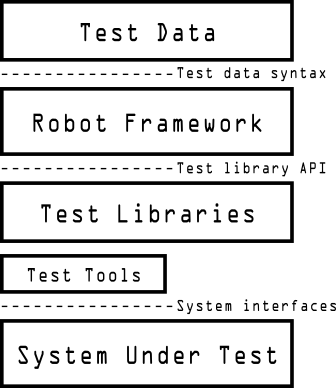
\includegraphics[width=0.4\textwidth]{assets/robot-arkkitehtuuri.png}
      \caption{Robot framework alustan arkkitehtuuri}
      \label{fig:robot-architecture}
    \end{figure}

    Robot frameworkillä rakennettuja testitapauksia voidaan ajaa komentoriviltä robot komennolla.
    Testitapauksien ajaminen tulostaa komentoriville yksinkertaisen raportin testitapauksen onnistumisesta ja lisäksi tallettaa varsin yksityiskohtaisen ja selkeän testitaportin ajetuille testitapauksille.
    Testiraportit ovat erittäin hyvin tehtyjä ja html-pohjaisia, joka tarkoittaa että ne voidaan helposti integroida osaksi jatkuvan integraation koontiputkia.

    Yhtenä heikkoutena Robot frameworkissa on tuen puuttuminen ohjelmistokieliperustaisissa testikehyksissä löytyville kontrollirakenteille, joita esiintyy esimerkiksi yksikkötestaukseen tarkoitetuissa testikehyksissä.
    Robot framework on selkeästi vain hyväksymistestauksen testitapauksien rakentamista varten tarkoitettu testialusta ja siinä se on erinomainen vaihtoehto testitapauksien rakentamiseen.

  \subsection{Selenium} \label{ch:08_selenium}

    % TODO: Kirjoita tämä kappale

    \begin{itemize}
      \item Mikä se on?
      \item Mihin sitä käytetään?
      \item Mitä hyötyjä siitä saadaan?
      \item Sisäinen rakenne / yksityiskohtainen esittely
      \item (Mitä heikkouksia siinä on?)
      \item Yhden lauseen yhteenveto
    \end{itemize}

  \subsection{Xvfb} \label{ch:08_xvfb}

    % TODO: Kirjoita tämä kappale

    \begin{itemize}
      \item Mikä se on?
      \item Mihin sitä käytetään?
      \item Mitä hyötyjä siitä saadaan?
      \item Sisäinen rakenne / yksityiskohtainen esittely
      \item (Mitä heikkouksia siinä on?)
      \item Yhden lauseen yhteenveto
    \end{itemize}

  \subsection{GoCD} \label{ch:08_gocd}

    % TODO: Kirjoita tämä kappale

    \begin{itemize}
      \item Mikä se on?
      \item Mihin sitä käytetään?
      \item Mitä hyötyjä siitä saadaan?
      \item Sisäinen rakenne / yksityiskohtainen esittely
      \item (Mitä heikkouksia siinä on?)
      \item Yhden lauseen yhteenveto
    \end{itemize}

  \subsection{Docker} \label{ch:08_docker}

    % TODO: Kirjoita tämä kappale

    \begin{itemize}
      \item Mikä se on?
      \item Mihin sitä käytetään?
      \item Mitä hyötyjä siitä saadaan?
      \item Sisäinen rakenne / yksityiskohtainen esittely
      \item (Mitä heikkouksia siinä on?)
      \item Yhden lauseen yhteenveto
    \end{itemize}

\section{Testitapauksien määrittäminen} \label{ch:08_testitapauksien_maarittaminen}

  Testitapaus on testiautomaation näkökulmasta, määritelty toimenpiteiden, ehtojen ja muuttujien joukko, joka suorittamalla voidaan verifioida ominaisuus tai toiminnallisuus ohjelmistosta.
  Testitapauksiin liittyy oleellisesti testikokoelman käsite, joka tarkoittaa samaan kontekstiin kuuluvista testitapauksista muodostettua joukkoa.
  Tässä diplomityössä keskitettyyn hyväksymistestaukseen liittyen testitapaukset kirjoitetaan usein käyttötapauksien muodossa.
  Lisäksi hyväksymistestauksen priorisoimiseen painotetun verkon avulla on suositeltavaa suunnitella ja rakentaa testitapaukset näkymä ja siirtymäperusteisesti, jotta matemaattisia verkkoja voidaan kunnolla hyödyntää.

  Testitapauksen perusformaatti koostuu lähtötilanteesta, laukaisijasta ja verifikaatiosta.
  Lähtötilanteessa oletetaan jotakin ja seuraavassa vaiheessa seurataan kun jokin ehto tapahtuu, jonka jälkeen voidaan tarkistaa seuraus ja verifioida onko se oletuksen mukainen.
  Testitapauksien yleisiä tavoitteita ovat: yksinkertaisuus, läpinäkyvyys, käyttäjätietoisuus, epätoistuvuus, olettamattomuus, kattavuus, tunnistettavuus, jälkensä puhdistava, toistettava, syvyyttömyys ja atomisuus.

  \noindent\begin{minipage}{\linewidth}
  \renewcommand{\lstlistingname}{Koodi}
  \lstinputlisting[
    caption={Esimerkki testitapauksesta Robot frameworkillä},
    label=code:robot-framework-testitapaus,
    numbers=left
  ]{assets/robot-framework-testitapaus.robot}
  \end{minipage}

  Robot Frameworkin perustaja on kirjoittanut laajan ohjeistuksen siitä, miten Robot Frameworkiä käyttäen luodaan hyviä testitapauksia \parencite{klarck_how-to-write-good-test-cases_2019}.
  Klärckin ohjeistuksen pohjalta on huomioitavaa erityisesti testikokoelmien, testitapauksien ja avainsanojen nimeäminen jonka kuuluisi olla selkeää, kuvaavaa ja ytimekästä.
  Dokumentaation määrää testitapauksissa tulisi rajoittaa, sillä hyvin kirjoitetut testitapaukset ovat Robot frameworkiä käyttäen selkeitä jo sellaisenaan.
  Dokumentaatiota kuuluisi lisätä lähinnä vain testikokoelmiin yleisellä tasolla.
  Testikokoelmat kuuluisi sisältää vain toisiinsa liittyviä testejä ja testitapauksien sekä avainsanojen tulisi olla sellaisinaan selkeästi ymmärrettäviä.
  Muuttujien käyttöä suositellaan kapsuloimaan pitkiä ja kompleksisia arvoja, mutta arvojen syöttäminen ja palauttaminen muuttujia hyödyntäen tulisi pitää pois testitapauksien tasolta.

\section{Priorisointiongelma} \label{ch:08_priorisointiongelma}

  Testitapauksien priorisointi on kustannussyistä tai resurssien optimoinnin kannalta erittäin tärkeää.
  Ohjelmistotestauksessa on hyvä tiedostaa, että ohjelmistotuotetta ei usein voida testata täydellisesti, joka nostaa esiin tarpeen tärkeimpien testitapauksien löytämisestä.
  Testitapauksia voidaan priorisoida monella tavalla, joihin tämä diplomityö tuo yhden uudenlaisen painottua verkkoa hyödyntävän lähestymistavan.

  \begin{itemize}
    \item Painotetun verkon hyödyntäminen
    \item Muut priorisointitavat
    \item heuristinen priorisointi
    \item moscow menetelmä
    \item 3-tasoinen priorisointimenetelmä (pakollinen/hyödyllinen/toivottu)
    \item pair-wise vertailu
  \end{itemize}